\documentclass[conference]{IEEEtran}
\usepackage{amssymb,amsmath,amsthm}
\usepackage{algorithm}
\usepackage{algpseudocode}
\usepackage{graphicx}
\usepackage{caption}
\usepackage{cite}
\usepackage{sidecap}
%\usepackage{arydshln}

\usepackage[dvipsnames]{xcolor}
\colorlet{lhue}{SpringGreen}
\colorlet{mhue}{WildStrawberry}
\colorlet{ghue}{CornflowerBlue}
\colorlet{vhue}{Goldenrod}
\usepackage[textsize=small,textwidth=15mm]{todonotes}
\setlength{\marginparwidth}{15mm}
\newcommand{\NDT}[1]{\todo[bordercolor=ghue,linecolor=ghue,color=ghue!40]{Tias: #1}}
\newcommand{\NDTi}[1]{\todo[inline,bordercolor=ghue,color=ghue!40]{Tias: #1}}
\newcommand{\NDB}[1]{\todo[bordercolor=mhue,linecolor=mhue,color=mhue!40]{Behrouz: #1}}
\newcommand{\NDBi}[1]{\todo[inline,bordercolor=mhue,color=mhue!40]{Behrouz: #1}}

\DeclareRobustCommand*{\IEEEauthorrefmark}[1]{%
  \raisebox{0pt}[0pt][0pt]{\textsuperscript{\footnotesize\ensuremath{#1}}}}

\newtheorem{theorem}{Theorem}
\newtheorem{definition}{Definition}

\begin{document}

\title{A Branch-and-Cut Algorithm for Constrained Graph Clustering}

\author{
  \IEEEauthorblockN{
    Behrouz Babaki\IEEEauthorrefmark{1}, 
    Dries Van Daele\IEEEauthorrefmark{1}, 
    Bram Weytjens\IEEEauthorrefmark{2,3,4,5}
    Tias Guns\IEEEauthorrefmark{1,6}}
    \IEEEauthorblockA{\IEEEauthorrefmark{1}Department of Computer Science, KU Leuven, Belgium}
    \IEEEauthorblockA{\IEEEauthorrefmark{2}Department of Microbial and Molecular Systems, KU Leuven, Belgium}
    \IEEEauthorblockA{\IEEEauthorrefmark{3}Department of Plant Biotechnology and Bioinformatics, UGent, Belgium}
    \IEEEauthorblockA{\IEEEauthorrefmark{4}Bioinformatics Institute Ghent, Belgium}
    \IEEEauthorblockA{\IEEEauthorrefmark{5}Department of Information Technology, IDLab, UGent, Belgium}
    \IEEEauthorblockA{\IEEEauthorrefmark{6}Department of Business Technology and Operations, VUB, Belgium}
}



% \author{\IEEEauthorblockN{Behrouz Babaki}
% \IEEEauthorblockA{Dept. Computer Science\\
% KU Leuven, Belgium}
% \and
% \IEEEauthorblockN{Dries Van Daele}
% \IEEEauthorblockA{Dept. Computer Science\\
% KU Leuven, Belgium}
% \and
% \IEEEauthorblockN{Bram Weytjens}
% \IEEEauthorblockA{Dept. Microbial and Molecular Systems, KU Leuven, Belgium\\
% \& Dept. Plant Biotechnology and Bioinformatics, UGent, Belgium\\
% \& Bioinformatics Institute Ghent, Belgium\\
% \& Dept. Information Technology, IDLab, UGent, Belgium}
% \and
% \IEEEauthorblockN{Tias Guns}
% \IEEEauthorblockA{Dept. Computer Science, KU Leuven, Belgium \\ \&
% Dept. Business technology and Operations, \\VUB, Belgium}}

\maketitle

\begin{abstract}
Clustering is a well-defined problem class in data mining, and many variations of it exists. However, practitioners often have additional constraints or quality scores that are not supported by standard algorithms. This has lead to the study of constrained clustering, which investigates generic methods to handle a variety of constraints and objectives. In our bioinformatics work, we were faced with exactly such a problem: a graph clustering problem with strict connectivity requirements and an objective function based on penalties rather than density of the clustering. In this paper, we explain the problem including the constraints and quality measures, and propose to use generic Mixed Integer Programming to solve it. We propose two approaches to handle the connectivity requirement in particular: one defined over all simple paths in the graph explicitly, and one based on cutting planes that enforce connectivity only when needed. Our experiments show that these approaches are able to solve the problem well. We hence demonstrate the applicability of generic OR methods on this application-driven data mining problem.
\end{abstract}

\section{Introduction}
\label{introduction}

% graph clustering (and partitioning)
Clustering is the task of partitioning a set of entities into
homogeneous subsets. The quality of the clustering is typically determined by the \textit{distance} between the entities. In graph clustering~\cite{schaeffer2007graph}, each entity is assumed to be a node in a graph; this graph is typically not fully connected. The quality is then determined by the \textit{density} of the entities within a cluster or by the \textit{cut size} between the clusters, that is the number of edges shared between different clusters. The latter is for example frequently studied in the field of graph partitioning~\cite{BulucMSS016}. Graph clustering has applications in many domains including social network analysis and community detection, information networks, transportation and logistics, and bioinformatics~\cite{schaeffer2007graph}.

% constrained clustering
As data mining is increasingly applied on more and more problems in different domains, it increasingly happens that existing clustering methods are not suited for the problem at hand. This is either because the problem domain imposes additional constraints that can not be expressed in these methods, or because the objective function has a non-standard form. This has lead to the field of \textit{constrained clustering}, which studies clustering problems involving different constraints and objectives~\cite{basu2008constrained}. An increasingly popular way to handle a broad range of constraints and objectives is to use generic optimisation tools. In other words, to cast the problem as an optimisation problem and to use generic (discrete) optimisation solvers such as constraint programming~\cite{DaoDV13}, mixed integer programming~\cite{DBLP:conf/aaai/GilpinND13,DBLP:conf/cpaior/BabakiGN14} or maximum satisfiability solvers~\cite{DBLP:journals/ai/BergJ17}. Though scalability can be an issue, these solvers can intrinsically handle different objectives and constraints.

% bio problem (interaction & co-occurence + size)
The problem we study in this paper is such a graph clustering problem that does not fit existing approaches. It is part of a bigger pipeline in computational cancer research, where the goal is to find \textit{pathways} in gene interaction networks. There is hence an \textit{interaction network} and it is a hard constraint that all nodes belonging to a cluster must be connected in this interaction network. To evaluate the quality there is a separate weighted \textit{co-occurence} network and the nodes belonging to a cluster should have a low co-occurence penalty. Furthermore, small pathways are biologically less meaningful and hence the size of the clusters should also be maximized. The problem is hence a bi-objective graph clustering problem with hard connectivity constraints on a separate network. Existing methods are not able to handle such a complex setting, hence we study a mixed integer programming approach.
%This perspective encourages formulating
%data mining problems as models in constraint satisfaction/optimization
%frameworks (e.g. constraint programming and integer programming). One
%of the motivations for doing so is that existing algorithms can be
%extended to new problems by modification of addition of constraints.

% contributions
More specifically, our contributions are as follows: 1) we identify a new bi-objective constrained graph clustering with applications in bio-informatics and present an MIP formulation of the problem; 2) in order to better handle the large number of connectivity constraints, we propose a branch-and-cut approach that adds connectivity constraints as needed using the principle of node-cut sets. Our experiments demonstrate the effectiveness of the approach.

The rest of this paper is structured as follows: we first discuss related work. In
section~\ref{sec:motivation} we present the application that motivates
this problem.  Section~\ref{sec:definition} introduces the formal
problem definition and a MIP formulation with the connectivity requirement.
In section~\ref{sec:connectivity}, we introduce two methods for handling the connectivity requirement, including a cutting plane approach. Section~\ref{sec:experiments} contains the experiments after which we conclude.


\section{Related work}
\label{sec:related}
There are several studies that apply mathematical programming to clustering and graph partitioning
problems~\cite{HansenJ97}. In addition to integer linear programming, semidefinite programming~\cite{ArmbrusterFHM08,LisserR03}, and quadratic programming~\cite{FanP10} formulations have also been used for solving these problems. Techniques such as branch-and-cut~\cite{FerreiraMSWW98,GrotschelW89} and branch-and-price~\cite{MehrotraT98,JiM07} have been used to improve the performance. 

There are several variants of the graph partitioning problem. When the underlying graph is a complete graph, this problem is sometimes called the \emph{clique partitioning} problem. In most variants of the graph partitioning problem, the edges, nodes, or both are weighted. The number of clusters can be specified by the user or they can be decided by the algorithm.The two most prominent types of objective functions are 1) the total weight of the edges that have endpoints in different clusters and 2) the total weight of the edges that have endpoints in the same cluster. Depending on the meaning of the weights, these function are minimized or maximized. In either case, these objectives are meant to increase the homogeneity of the clusters.

Several types of constraints are common to the graph partitioning problem. The most widely used constraint is the \emph{balance} constraint that requires the number of nodes in all clusters to be almost equal~\cite{LabbeO10}. Other types of constraints include constraints on the size of clusters~\cite{FanP10}, and constraints on the total weight of nodes in a cluster~\cite{FerreiraMSWW98}. 

The main difference of our problem with existing ones is that we have two graphs, where the edges of the co-occurrence graph are weighted, but the goal is to minimize their total value. The connectivity of the nodes in the interaction network are required and must hence be added as hard constraints. The graph partitioning problem of \cite{Benati2017} also requires such constraints. However, they do not assume that the number of clusters is given, and their encoding of the clustering problem is quite different from ours. 

\section{Motivating application}
\label{sec:motivation}
In cancer research, tumor tissue is collected from patients for further study. Such a tumor is basically a cell in which one or more genes have mutated. Normally that cell would be destroyed by the immune system, but in case of a tumor that cell has managed to survive and may even be growing (out of control).
Genes and mutated genes can be identified in a tumor by sequencing the DNA of the tissue. Nowadays, this sequencing has become fairly commonplace, enabling the genome-wide measurement of mutated genes across large groups of cancer patients.

The key challenges when interpreting these data are to detect the (mutated) genes that affect the creation and development of cancer and to gain an understanding of their interaction. Initially, the main focus by the community was solely on the detection of key driver genes. However, there are typically many mutated genes making it challenging to detect rare ones with high statistical significance. For this reason, there is recently a rise in methods aiming to exploit the information contained in the human interaction network \cite{leiserson2015pan,pulido2015ssa}. This network expresses which genes interact with each other. This can be used to verify that a set of genes interact with each other.

In our setting we start by considering a subgraph of the human interaction network containing only those genes and interactions that were identified as being highly relevant to breast cancer. Each node represents a gene or gene product, and each edge represents an interaction between a pair of nodes. The graph may consist of multiple connected components. It is our goal to separate distinct \textit{pathways} from each of these components, where a pathway is a set of genes that interact with each other.

By incorporating such biological pathway information, a superior selection and understanding of genes and their interactions is possible. %These new methods do introduce novel challenges. We notice that the underlying mechanisms that affect individual patients are not always easily distinguishable from the extracted subgraphs. More specifically, it is the case that the pathways contained in these subgraphs may be connected to one another or even overlap.
%
A difficult challenge however is how to determine that two genes are more likely to belong to the same or to a different pathway. Fortunately, it is known that the creation and growth of tumors follows a clonal \textit{evolutionary} model. Following this model, it is considered unlikely that a tumor would disrupt and mutate different genes within a single pathway. Indeed, it is sufficient to disrupt one gene to disrupt the pathway, and hence evolutionarily there is little incentive to disrupt others as well. As a consequence, it is less common that multiple mutated genes of a single pathway are observed within the same patient. We can hence compute a co-occurrence penalty score for each pair of genes, based on the harm associated with the mutations and the number of patients for whom that pair was observed.

While obtaining pathways with a low penalty is important, one should not go as far as dividing the genes into small clusters. For this reason, we will aim to balance the size of the (smallest) pathway with the amount of penalty the pathways incur.



\begin{figure}
\centering
\begin{minipage}{.3\linewidth}
\centering
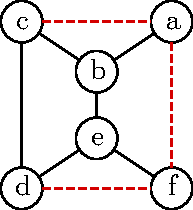
\includegraphics[scale=0.6]{images/interaction}
\end{minipage}%
\begin{minipage}{.3\linewidth}
\centering
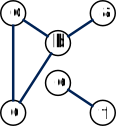
\includegraphics[scale=0.6]{images/interaction_no_overlap}
\end{minipage}%
\begin{minipage}{.4\linewidth}
\centering
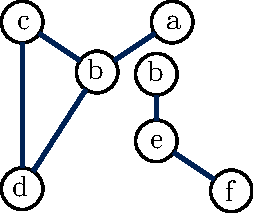
\includegraphics[scale=0.6]{images/interaction_overlap}
\end{minipage}
\captionsetup{font=small,margin=10pt}
\captionof{figure}{(left) A small subgraph extracted from the interaction network. Dashed lines represent the can-not-link constraints. (middle) the pathways obtained from non-overlapping clusters (right) the pathways obtained from overlapping clusters.}
\label{fig:minimal}
\end{figure}


\section{Problem and MIP formulation}
\label{sec:definition}

From a computational point of view, the input to our problem are a set of genes and two graphs over those genes: an unweighted interaction graph and a weighted co-occurrence graph. We first review some basic graph concepts before formally defining the problem.

A graph $G=(V, E)$ consists of a set of nodes $G$ and a set of edges $E$. Each edge $e \in E$ is a tuple $(u,v), u,v \in V$ and the graph is \textit{undirected} if the ordering of the edges does not matter. The graph is \textit{weighted} if each edge $e \in E$ has a corresponding weight $w(e)$.
A graph is \emph{simple} if it does not have any loops or double edges.
A graph is \emph{connected} if there is a path between each pair of its nodes. The nodes on a path except the first and last ones are called the \emph{intermediate nodes}. A \emph{simple path} is a path with no cycles. Another important concept is that of an induced subgraph. Given a set of nodes $V' \subseteq V$, the \textit{ induced subgraph} of $G$ on $V'$ is a graph $G[V']$ that contains only the nodes in $V'$ and only the edges of $G$ that have both endpoints in $V'$. 

\subsubsection{Problem definition}
Our problem is as follows: given a set of genes $V$, a simple undirected graph $G_i=(V,E_i)$ representing the interaction network and a simple weighted undirected graph $G_o=(V,E_o)$ with weight function $w_o$ representing the co-occurence network. The goal is to partition $V$ into $k$ different groups $V_1,\ldots,V_k$, where $k$ is assumed given. Each cluster induces a subgraph on the interaction graph $G_i$ and that subgraph \textit{must be connected}. The quality of a clustering is determined by the size and co-occurence penalty of the clusters. The two are linearly combined using $\gamma$ to obtain the following objective that must be maximized:
\begin{equation}
f(V_1,\ldots,V_k) = min_{c=1}^{k} |V_c| - \gamma \sum_{c=1}^{k} \sum_{e \in G_o[V_c]} w_o(e) \label{eq:def}
\end{equation}
The first component represents the size of the smallest cluster while the second component represents the sum of weighted edges in the induced subgraph of the co-occurence graph $G_o$ on the cluster $V_c$. $\gamma$ can be used to balance the size component to the co-occurence penalty computed and is assumed given.

%Consider a simple undirected graph $G=(V, E)$ where nodes represent genes, and edges represent interactions between those genes. Our goal is to partition $V$
%into $k$ subsets (called \emph{clusters} from now on), such that the
%subgraph induced by each subset is connected. These represent the pathways we seek to identify. Our preference is to avoid
%having clusters that contain only a small number of nodes. To enforce
%this preference, we define one of our goals as maximizing the size of
%the smallest cluster. Moreover, there exists a set of tuples
%$C = \{(u, v, w): u, v \in V, w \in \mathbb{R}^+\}$ which indicates that
%including $u$ and $v$ in the same cluster will induce a penalty of $w$. We denote all edges $(u, v)$ such that $(u, v, w) \in C$ by $E_C$. Our second goal is to minimize the sum of such penalties.
%
%
%To include both goals in the objective function, assume that $S$ is the
%size of the smallest cluster and $W$ is the total penalty. We define the
%objective function as maximizing $S - \gamma W$ where $\gamma$ is a
%positive parameter specified by user which determines the relative importance of each of the two goals.


\subsubsection{Mixed integer programming}
We can formulate this problem as an integer linear program. The main
decision variables in this formulation are those that determine the
assignment of nodes to the clusters. We will use binary variables $x_{ic}$ indicates whether or not node $i$ is included in
cluster $c$. Each cluster must be assigned to exactly one cluster. This can be enforced by the following set of constraints:
%
\begin{equation}
\sum_{c=1}^k x_{ic} = 1 \quad \forall i \in \{1, \ldots, |V|\} \label{cons:assign}\\
\end{equation}

To model the first component of the objective in Eq.~\ref{eq:def} we introduce an integer variable $s$ which represents the size
of the smallest cluster. The domain of $s$ is
$\{0, \ldots, \lfloor \frac{|V|}{k} \rfloor \}$. The following constraints
ensure that $s$ is smaller or equal than the size of each cluster.
%
\begin{align}
s \leq \sum_{i=1}^{|V|} x_{ic} \quad \forall c \in \{1, \ldots, k\}
\end{align}
As $s$ is included in the objective function it will be maximized and hence take the value of the size of the smallest cluster during optimisation.


For the second component, we introduce additional variables to model the edges in the induced subgraph $G_o[V_c]$ of each cluster. More specifically, we introduce binary variables $y_{ijc}$ which are equal to one if and only if
nodes $i$ and $j$ are both included in cluster $V_c$. To enforce
this property, we add the following constraints to the model:
\begin{equation}
y_{ijc} \geq x_{ic} + x_{jc} -1 \quad \forall c \in \{1, \ldots, k\}, \forall (i,j) \in E_o
\end{equation}
When both $x_{ic}$ and $x_{jc}$ are equal to one, this constraint forces
$y_{ijc}$ to be equal to one. Otherwise, $y_{ijc}$ can be either zero or
one. However, as we will see, $y_{ijc}$ is included in the objective
function with a negative coefficient. Hence the optimization procedure
will automatically fix $y_{ijc}$ to zero in such cases.

Our formulation so far does not ensure that the nodes in each cluster
are connected. For now assume that constraint
$\mathsf{connected}(x_{1c}, \ldots, x_{|V|c})$ enforces the connectivity of
cluster $c$. We will discuss the exact formulation of this constraint in
the next section. 

The complete model that we defined is hence the following, where $w_o((i,j)) = w_o(e)$ for $e=(i,j)$:
\begin{align}
& \text{maximize} \quad s - \gamma \sum_{c=1}^{k} \sum_{(i,j) \in E_o} w_o((i,j))* y_{ijc}  \\
&\textit{s.t.}                                                                       \nonumber \\
&\sum_{c=1}^k x_{ic} = 1                                                            \quad \quad \forall i \in \{1, \ldots, |V|\} \\
& y_{ijc} \geq x_{ic} + x_{jc} -1                                                    \quad \quad \forall c \in \{1, \ldots, k\}, \forall (i,j) \in E_o \\
& s \leq \sum_{i=1}^{|V|} x_{ic}                                                   \quad \quad \forall c \in \{1, \ldots, k\} \\
& \mathsf{connected}(x_{1c}, \ldots, x_{|V|c})                                       \quad \quad \forall c \in \{1, \ldots, k\} \\
& x_{ic} \in \{0, 1\}                                                                 \quad \quad \forall c \in \{1, \ldots, k\}, \forall i \in \{1, \ldots, |V|\} \\
& y_{ijc} \in \{0, 1\}                                                               \quad \quad  \forall c \in \{1, \ldots, k\}, \forall (i, j) \in E_o \\
& s \in \{0, \ldots, \lfloor \frac{|V|}{k} \rfloor \}                                  
\end{align}

\section{Extensions and improvements}
We choose to use a generic discrete constraint solver to solver our non-traditional clustering problem. In the following we discuss three extensions to the above formulation that are possible thanks to the use of generic solvers and there ability to handle different types of constraints.


\subsection{Overlapping clusters}
It is known that genes can occur in multiple pathways, and hence we may wish to allow for nodes to be included in more than one cluster.
To apply this modification to our formulation, we only need to replace constraints~\eqref{cons:assign} with the following inequalities:
%
\begin{equation}
\sum_{j=1}^{k} x_{ij} \geq 1 \qquad i \in \{1, \ldots, |V| \}
\end{equation}
%
\subsection{Breaking symmetries}
Clustering problems often have an inherent symmetry which is due to the fact that the labels of clusters are arbitrary. This means that for each solution, there are $k!$ equivalent solutions that only differ by the cluster labels. We can strengthen our formulation by breaking these symmetries. \cite{SheraliD05a} suggests two measures to reduce these symmetries: 1) assign label $1$ to the cluster that contains node $1$. 2) assign labels to other clusters in the increasing order of their sizes. This translates to the following constraints:
%
\begin{align}
&x_{11} = 1 \\
&\sum_{i=1}^{|V|} x_{ic} \leq \sum_{i=1}^{|V|} x_{i(c+1)} \qquad c \in \{2, \ldots, k-1\}
\end{align}

These constraints do not eliminate all symmetries (especially in the case of overlapping clusters) but still lead to improvements in performance in practice. 

\subsection{Obtaining the set of Pareto optimal solutions} \label{sec:pareto}
In the above formulation we used the commonly employed method of reducing a bi-objective optimisation problem to a single-objective one through the use of a balancing parameter $\gamma$. An alternative solution is to use a bi-objective optimisation approach to compute the set of \emph{Pareto optimal} solutions. A solution of a bi-objective optimization problem is Pareto optimal if there is no other solution with a better quality with respect to both objectives. Obtaining the set of Pareto optimal solutions for other types of bi-objective constrained clustering has been studied before~\cite{GunsDVD16}. As in that work, we use a method based on the $\epsilon$-constraint algorithm~\cite{DBLP0015143} to obtain the Pareto optimal solutions. To do this, we remove the size component from the objective leaving only the co-occurence part. Then we iteratively solve this modified problem, each time adding a constraint such that the size of the smallest cluster is larger than that found in the previous iteration ($m$):
%
\begin{align}
\sum_{i=1}^{|V|} x_{ic} > m \quad \forall c \in \{1, \ldots, k\}
\end{align}
The approach is depicted in Algorithm~\ref{alg:pareto}.

\begin{algorithm}[t]
\centering
\caption{Computing the set of Pareto optimal solutions}
\label{alg:pareto}
\begin{algorithmic}[1]
\State $\mathcal{P} \gets \emptyset$ \Comment{the set of Pareto optimal solutions}
\State $m \gets 0$ \Comment{Minimum size of the previous solution}
\Repeat
	\State $solution \gets \textsc{MinimizePenalties}(V, G_i, G_c, k, m)$
	\State $\mathcal{P} \gets \mathcal{P} \cup solution$
	\State $m \gets$ size of the smallest cluster in $solution$
\Until{no $solution$ was found}
\State \Return $\mathcal{P}$
\end{algorithmic}
\end{algorithm}

%\NDTi{possible story: 1) ensure connectedness: must be a path between two coclustered poins; 2) cutting plane is generate when violated. Generating 17 requires adding 16's too. Instead, can use relation between connectedness and node-cuts. Using node-cuts in constraints is over variables directly. Number of node-cuts is worst-case exponential, but one violated one is sufficient to invalidate a solution so can generate one as cutting plane. Which one? For integer values does not matter: any violated one. Common approach to finding node-cuts is using a flow problem. Can use this here as follows... Advantage of solving flow problem is that also applicable to real-valued xs. Hence algorithm is...}
\section{Enforcing connectivity}
\label{sec:connectivity}

The remaining issue to work out is how to represent the $\mathsf{connected}(x_{1j}, \ldots, x_{|V|j})$ constraint. We investigate two different approaches.

For a cluster to be connected, there should exist for each pair of points belonging to the cluster at least one path between these two nodes such that all nodes on this path also belong to the cluster. In section~\ref{sec:enumerate} we enforce this condition by explicitly enumerating all simple paths between each pair of non-adjacent nodes in the graph and adding variables and constraints for these paths. However, the total number of paths can be exponential leading to very large models to solve.

A way to avoid having to ground out constraints for all the possible paths is to incrementally add only those constraints needed. The \emph{cutting plane} algorithm is a method that allows this exactly. In section~\ref{sec:bnc} we introduce another formulation for the connectivity constraint based on node-cut sets, which also has a worst-case exponential number of constraints but which lends itself well to an incremental cutting plane method.

\subsection{Enumerating all simple paths}
\label{sec:enumerate}

Consider a simple path between the nodes $u$ and $v$. Let $I$ denote the set of indices of the intermediate nodes on this path. Assume that binary variable $y_c$ indicates that all these nodes belong to cluster $c$. A standard translation of the relation $(y_c=1) \Leftrightarrow \land_{i \in I} (x_{ic}=1)$ to linear constraints gives the following inequality:
%
\begin{equation*}
0 \leq \sum_{i \in I} x_{ic} - |I|y_c \leq |I|-1
\end{equation*}

In general, let $P_{uv}$ denote the set of all simple paths between nodes $u$ and $v$ in the interaction graph. For a path $P_r \in P_{uv}$, let $I_r$ denote the set of indices of intermediate nodes of $P_r$. We introduce binary variable $y_{rc}$ to indicate that all these nodes are assigned to cluster $c$. This relationship is enforced by the following constraints:
\begin{multline}
0 \leq \sum_{i\in I_r} x_{ic} - |I_r| y_{rc} \leq |I_r| - 1 \qquad \forall u, v \in V, (u, v) \notin E, \\
\forall r \in \{1, \ldots, |P_{uv}|\}, \forall c \in \{1, \ldots, k\}
\label{cons:path}
\end{multline}
%  -- implicit: |I_r| will be 0 in that case.

Finally, to enforce the condition $(x_{uc}=1 \land x_{vc}=1) \Rightarrow \lor_{r} (y_{rc}=1)$, we add the following constraints to the model:
%
\begin{multline}
x_{uc} + x_{vc} -1 \leq \sum_{r=1}^{|P_{uv}|} y_{rc} \qquad
\forall u, v \in V, (u, v) \notin E, \\ \forall c \in \{1, \ldots, k\}
\label{cons:pconnect}
\end{multline} 

These constraints ensure there exists at least one path in the interaction graph between every two nodes in the same cluster.

\subsection{A cutting plane approach}
\label{sec:bnc}

 In the cutting plane method two steps are iteratively repeated: 1) A model that includes only a subset of the constraints is solved. 2) A constraint that is violated by the current solution, a cut, is added to the model. These steps are repeated until no constraint is violated. To use the cutting plane algorithm, we need an oracle that given an assignment $\mathbf{x}$ can check if $\mathbf{x}$ satisfies all constraints and if not, finds a constraint that is violated by $\mathbf{x}$. Since in the latter case the added constraint separates $\mathbf{x}$ from the feasible region, the problem solved by the oracle is called the \emph{separation} problem.
 In a \emph{branch and cut} algorithm, cutting planes are added throughout the branch and bound tree. 
 
 %\NDT{removed a sentence about LP relaxation, too early and I don't get it ; )} %Note that even if we add some or none of the cuts to the linear programming (LP) relaxation, it will still provide a valid bound. Hence it is possible to add the cuts only when an integer solution is obtained.

 A cutting plan approach with the formulation of connectivity from the previous section would require us to add both variables (the $y_{rc}$ ones) and constraints \eqref{cons:path} and \eqref{cons:pconnect} for each cut.
% Applying the cutting plane method to the formulation of connectivity in the previous subsection is not easy, since the $y$ variables in a constraint from the constraint set~\ref{cons:pconnect} couple it with an exponential number of constraints from the constraint set~\ref{cons:path}.
Instead, we adopt the approach of ~\cite{CarvajalCGVW13} which defines the connectivity constraints in terms of \emph{node-cut sets}. The advantage is that no extra variables need to be introduced, and that between two nodes the connectivity can be broken incrementally with individual constraints. The following definition and theorem are taken from~\cite{CarvajalCGVW13}.

\begin{definition}[Node-cut set]
Given nodes $u, v \in V$ that are not adjacent ($(u, v) \notin E$), a set of nodes $S \subseteq V \setminus \{u, v\}$ is a \emph{node-cut set} separating $u$ and $v$ (or simply a \emph{$uv$-node cut}) if all paths between $u$ and $v$ intersect $S$.
\end{definition}
There is hence at least one node from every path between $u$ and $v$ in the $uv$-node cut.
A $uv$-node cut is \emph{minimal} if it is not a $uv$-node cut after removing any of its nodes. For a pair of non-adjacent nodes $u$ and $v$, we denote by $\Gamma(u, v)$ the set of all minimal $uv$-node cut sets. Figure~\ref{fig:cutset} shows examples of minimal node-cut sets. The following theorem relates the connectivity of a graph to its minimal node-cut sets. 
%
\begin{SCfigure}[1.2]
\centering
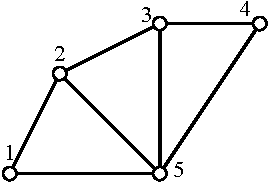
\includegraphics[scale=0.7]{images/cutset}
\captionsetup{font=small}
\captionof{figure}{The sets \{2, 5\} and \{3, 5\} belong to $\Gamma(1, 4)$, but the set \{2, 3, 5\} does not because it is not minimal.}
\label{fig:cutset}
\end{SCfigure}
%
\begin{theorem}
Given $U \subseteq V$ and a pair of non-adjacent nodes $u, v \in U$, there exists a path between $u$ and $v$ in the subgraph induced by $U$ if and only if all $uv$-node cuts $S$ are such that $S \cap U \neq \emptyset$.
\label{theorem:cutset}
\end{theorem}
%
For every $uv$-node cut $S$ this theorem states thatto ensure that cluster $c$ is connected, at least one node in the node cut must belong to the cluster:
%
\begin{equation*}
(x_{uc}=1 \land x_{vc}=1) \Rightarrow \lor_{w \in S} (x_{wc}=1)
\end{equation*}

By translating this condition into linear constraints we can formulate the constraint $\mathsf{connected}(x_{1c}, \ldots, x_{|V|c})$ as follows:
%
\begin{multline}
\sum_{w \in S} x_{wc} \geq x_{uc} + x_{vc} - 1 \\
\forall (u, v) \in V, (u, v) \notin E, S \in \Gamma(u, v)
\label{eq:connectivity}
\end{multline}

The constraint set~\eqref{eq:connectivity} contains an exponential number of constraints. Following the cutting plane method, we will iteratively add some of the violated constraints to the model. A common practice is to add one or some of the constraints \emph{most violated} by the current solution in each iteration.

Given a solution $\mathbf{x}^*$ of the problem, let us denote the value of $x_{ic}$ variables in this solution by $x^*_{ic}$ and the vector of variables corresponding to cluster $c$ by $\mathbf{x}^*_c$.
In this respect, a first observation is that $\sum_{w \in S} x^*_{wc} \geq 0$ is always true as the $x^*$ are Boolean variables. Hence, the constraint can only be violated if $x^*_{uc} + x^*_{vc} - 1 > 0$, that is, if both variables belong to the same cluster. If that is the case, then the constraint can only be violated if $\sum_{w \in S} x^*_{wc} = 0$, that is, if none of the nodes in the cut set are in the cluster. If no such constraint can be found that the connectivity constraint is satisfied.

The same principle can be used on real-valued solutions (as computed by the MIP solver when solving the linear relaxation). The most violated constraint for a non-adjacent pair $(u,v)$ is now the constraint for which $x^*_{uc} + x^*_{vc} - 1 > 0$ and that minimizes $\sum_{w \in S} x^*_{wc}$. To add a cut of $(u,v)$ in the cutting plane algorithm, the goal is hence to find the node-cut set $S^*$,
\begin{equation}
S^* =\underset{S \in \Gamma(u, v)}{\mathrm{argmin}} \sum_{w \in S} x^*_{wc}
\label{eq:separation}
\end{equation}
%If $\sum_{w \in S^*} x_{wc}^* < x^*_{uc} + x^*_{vc} - 1$ then the equality~\ref{eq:connectivity} induced by $u, v, S^*$ is violated. If no such violated constraint is found, then the solution is optimal.

It is shown in~\cite{CarvajalCGVW13} that the solution for equation~\ref{eq:separation} can be computed efficiently: If we use $x^*_{ic}$ as the capacity of node $i$, the separation problem reduces to finding the minimum capacity node cut separating $u$ and $v$. This problem can be solved using any standard \emph{min-cut} algorithm. A summary of the cut generation procedure is presented in algorithm~\ref{alg:cut}, where for each cluster the most violated constraint among its node-pairs is added.

\begin{algorithm}
\centering
\caption{The cut-generation procedure}
\label{alg:cut}
\begin{algorithmic}[1]
\State $\mathcal{C} \gets \emptyset$ \Comment{Set of constraints to add}
\For{$c \in \{1, \ldots, k\}$}
	\For{$u, v$ such that $(u, v) \notin E_i$ and $x_{uc}^* + x_{vc}^* > 1$}
		\State $S^* \gets \text{min-cut}(u, v, {\mathbf{x}}^{*}_c, G_i)$
		\State $\mathcal{C} \gets \mathcal{C} \cup \{\sum_{w \in S^*} x_{wc} \geq x_{uc} + x_{vc} - 1\}$
	\EndFor
\EndFor
\State Add constraints $\mathcal{C}$ to the model
\end{algorithmic}
\end{algorithm}





\section{Experiments}
\label{sec:experiments}
%
%In this section we will evaluate the suitability of our algorithms to address the motivating application. In particular, we want to answer these three questions:
%
%\begin{description}
%\item[Q1.] How does each of the two models scale in the task of overlapping clustering?
%\item[Q2.] How does each of the two models scale in the task of non-overlapping clustering?
%\item[Q3.] What is the effect of the $\gamma$ parameter on the trade-off between the two components of the objective function?
%\end{description}
%
%
%\subsection{Experiment setting}
We ran experiments on quad-core Linux machines with 32 GB of memory. We implemented our branch-and-cut algorithm using the Python interface
of \emph{Gurobi-7}\footnote{www.gurobi.com} and allowed it to use all 4 cores. The code and data are available online~\footnote{https://github.com/Behrouz-Babaki/graph\_clustering}.

To solve the separation problem, we used the min-cut/max-flow algorithm from the \emph{NetworkX-1.11} library~\cite{NetworkX}. In order to use this algorithm, we first replaced
each undirected edge by two opposite directed edges of infinite capacity.
Then, we replaced each node $v$ by two nodes $v_{\text{in}}, v_{\text{out}}$ connected by two opposite
edges, with capacities equal to the capacity of $v$. We obtain the
minimum node cut separating $u$ and $v$ by computing the minimum cut
between $u_{\text{out}}$ and $v_{\text{in}}$ in this graph.

We followed the recipe of~\cite{CarvajalCGVW13} for adding the cuts: cuts to the
linear relaxation were only added at the root node of the branch-and-cut tree.
Moreover, when adding cuts to the relaxation, we monitored the change in
the value of the objective function. If this value improved less than 5\% in 10 consecutive rounds, we stopped adding cuts. Outside the root node, we only add cuts when an integer solution is found. We normalized the two components of the objective function. We multiplied the size variable by $1/n$ in overlapping clustering and by $k/n$ in non-overlapping clustering. We divided the second component by the sum of edge weights.


The graphs used in our experiments were extracted from the HINT+HI2012 protein-protein interaction network~\cite{das2012hint,yu2011next}. We consider this selection of subgraphs representative of the graphs encountered in our application domain. Table \ref{table:instanceInformation} highlights some of the properties of our selected instances. Several of these instances contain a very low number of edges compared to nodes. As a direct result of this, they contain a very small number of paths. We have also selected a few graphs that contain more paths. These graphs also have a number high-degree nodes. Such hubs are fairly common in scale-free networks, of which protein-protein interaction networks are a common example.


%cite (High-quality protein interactomes and their applications in understanding human disease.  and Next-generation sequencing to generate interactome datasets. )
%


\begin{table}
\centering
\captionsetup{font=small}
\captionof{table}{instance properties}
\label{table:instanceInformation}
\begin{tabular}{|l c c c|}
\hline
\textbf{instance} & \textbf{\#simple paths} & \textbf{\#nodes} & \textbf{\#edges}\\
\hline
\texttt{200\_1000} & 93 & 40 & 46\\
\texttt{200\_1250} & 1508 & 52 & 68\\
\texttt{250\_750} & 45 & 30 & 32\\
\texttt{250\_1000} & 1040 & 69 & 81\\
\texttt{300\_750} & 59 & 44 & 46\\
\texttt{350\_500} & 12 & 13 & 12\\
\texttt{350\_750} & 73 & 58 & 60\\
\texttt{450\_750} & 105 & 90 & 92\\
\hline
\end{tabular}
\end{table}

\subsection{Results and discussion}
\subsubsection{Scalability of the two approaches}
We compare the runtime of the model formulation using all paths (ENUM) with that of using branch-and-cut (BNC), for a number of datasets and $k$ values and averaged over $\gamma\in\{0.1,0.25,0.33,0.5,1,2,3,4,5,10\}$. Table~\ref{table:runtime} shows the results. In each instance, one of the algorithms outperforms the other one. This divides the instances into two groups. Instances for which enumerating all paths has a better performance are those which have a similar number of nodes and edges (see table~\ref{table:instanceInformation}). As a result, the total number of simple paths in these graphs is small and the optimization model has a reasonable size. On the other hand, for two of the instances the branch-and-cut method provides a clear advantage. The total number of simple paths for these instances is considerably larger than the others. Hence, for these instances the extra effort for solving the separation problem pays off.

\subsubsection{Impact of $\gamma$}
The $\gamma$ parameter is a way of balancing the minimum size of the clusters with the total co-occurrence penalty. We showcase the effect of the parameter on these two components of the objective in Figure~\ref{fig:gamma} for instance \texttt{250\_750}. As $\gamma$ approaches $0$ most weight is given to the size leading to increasing larger minimum clusters but also a sharp incline in the total co-occurence penalty. For too high $\gamma$ values, $\geq 4$ in this case, the size of the clusters can drop to values of 1 or 2, which are not meaningful. In this case, a $\gamma$ between 1 and 3 seems most sensible.

\begin{figure}[b]
\centering
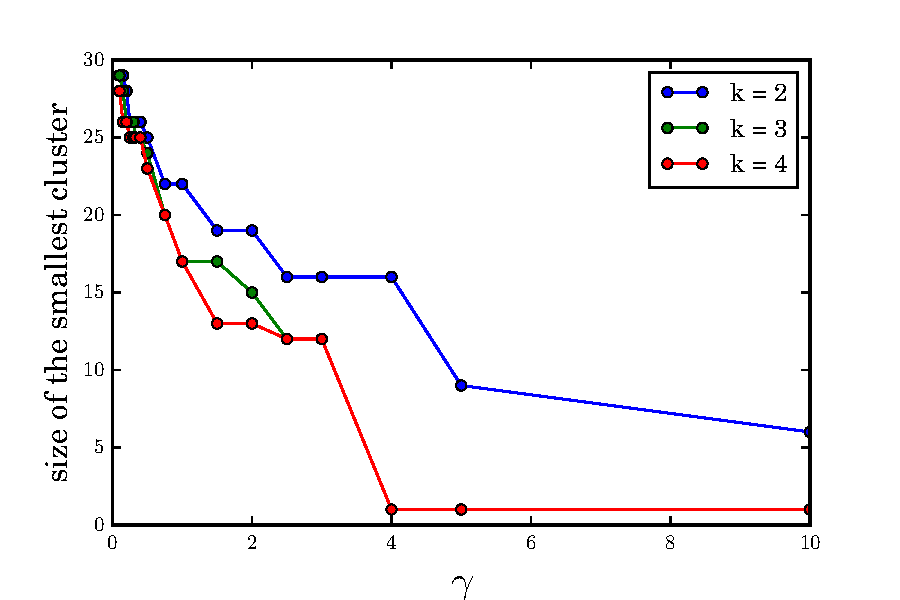
\includegraphics[scale=0.28]{images/clsize}
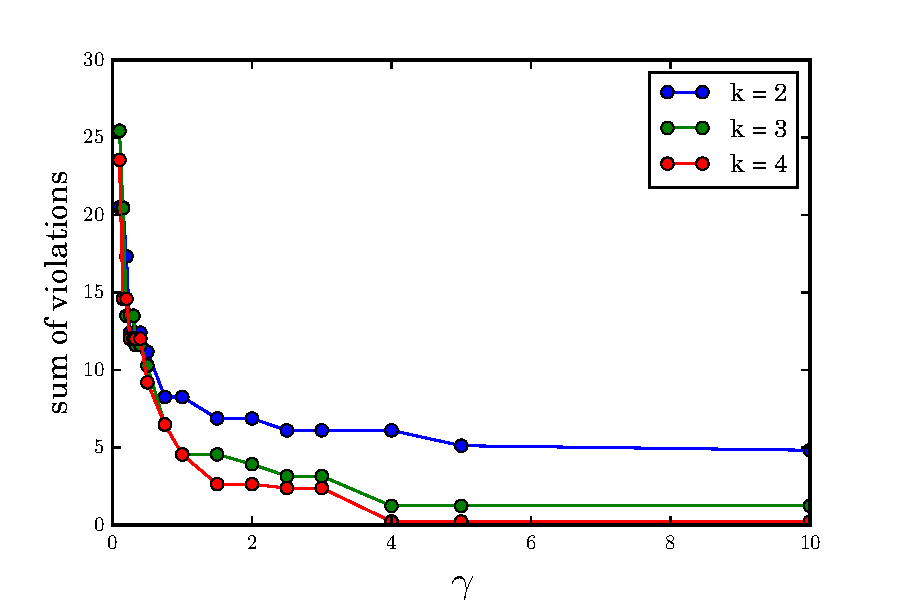
\includegraphics[scale=0.28]{images/penalty}
\captionsetup{font=small}
\caption{impact of $\gamma$ on smallest cluster size (left) and total co-occurrence penalty (right) for instance \texttt{250\_750}.}
\label{fig:gamma}
\end{figure}

\subsubsection{Pareto optimal set}
As explained in Section~\ref{sec:pareto} one can also use generic solvers to compute the Pareto-optimal set directly instead of having to determine a $\gamma$ parameter. In Figure~\ref{fig:pareto} for the non-overlapping setting we can see that a few smallest cluster values are skipped because not optimal, and that the there is a gradual increase in total violations as the minimum size increases, with an increase in incline near the end (there are 30 genes in this dataset). This can be used to select an appropriate solution among the Pareto optimal ones.

\begin{figure}
\centering
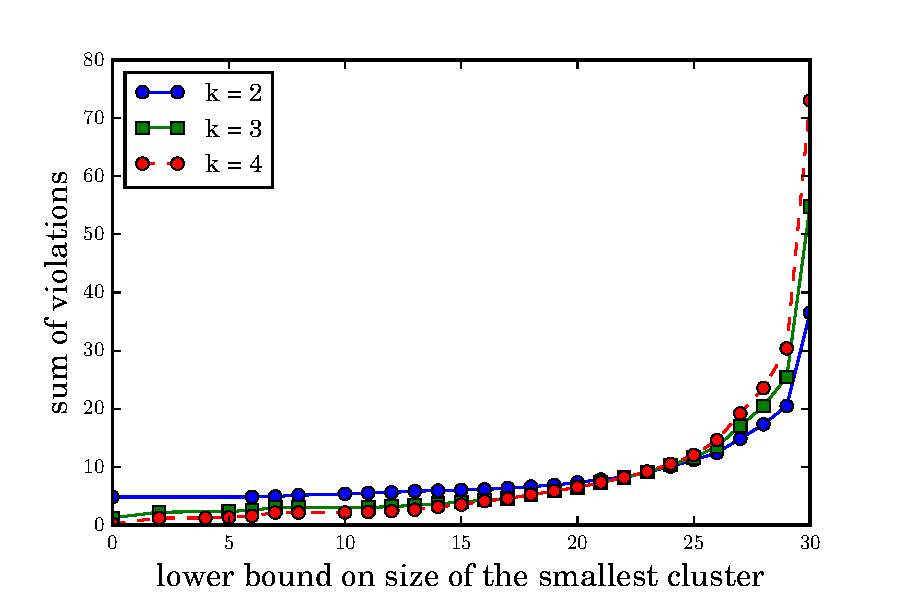
\includegraphics[scale=0.5]{images/pareto}
\captionsetup{font=small}
\caption{The Pareto optimal set for overlapping clustering on instance \texttt{250\_750} with three values for number of clusters.}
\label{fig:pareto}
\end{figure}




\begin{table}
\centering
\captionsetup{font=small}
\captionof{table}{Average runtimes of overlapping and non-overlapping clustering by enumerating all simple paths (AllPaths) and branch and cut (BnC). Timed-out experiments are counted as 600 seconds (--).}
\label{table:runtime}

\begin{tabular}{|ll|rr|rr|}
\hline
		 &   &  \multicolumn{2}{|c|}{\emph{overlapping}} & \multicolumn{2}{|c|}{\emph{non-overlapping}} \\
         \cline{3-6}
\emph{instance} & \emph{k} &  \emph{AllPaths} &  \emph{BnC} &  \emph{AllPaths} &  \emph{BnC} \\
\hline      
\texttt{200\_1000} & 2 &       \textbf{0.830} &    12.320 &      \textbf{0.319} &    13.398 \\
         & 3 &       \textbf{3.211} &    16.255 &       \textbf{4.474} &    15.007 \\
         & 4 &      \textbf{14.846} &    28.714 &      \textbf{15.578} &    52.262 \\
\hline         
\texttt{200\_1250} & 2 &     225.735 &    \textbf{43.740} &     113.210 &    \textbf{38.849} \\
         & 3 &     582.541 &    \textbf{52.950} &     298.390 &    \textbf{72.643} \\
         & 4 &         -- &   \textbf{188.287} &     595.930 &   \textbf{205.454} \\
\hline         
\texttt{250\_1000} & 2 &     487.222 &    \textbf{78.243} &     370.898 &    \textbf{69.481} \\
         & 3 &     587.700 &   \textbf{121.677} &         -- &   \textbf{217.079} \\
         & 4 &         -- &   \textbf{206.952} &         -- &       -- \\
\hline         
\texttt{250\_750} & 2 &       \textbf{0.166} &     4.058 &       \textbf{0.025} &     3.873 \\
         & 3 &       \textbf{0.321} &     6.433 &       \textbf{0.387} &     3.965 \\
         & 4 &       \textbf{0.737} &    10.564 &       \textbf{0.698} &     7.374 \\
\hline         
\texttt{300\_750} & 2 &       \textbf{0.333} &    12.232 &       \textbf{0.209} &    10.546 \\
         & 3 &       \textbf{0.761} &    20.365 &       \textbf{0.812} &    16.924 \\
         & 4 &       \textbf{1.728} &    28.267 &       \textbf{3.598} &    50.836 \\
\hline         
\texttt{350\_500} & 2 &       \textbf{0.004} &     0.093 &       \textbf{0.003} &     0.151 \\
         & 3 &       \textbf{0.006} &     0.129 &       \textbf{0.021} &     0.257 \\
         & 4 &       \textbf{0.007} &     0.181 &       \textbf{0.039} &     0.211 \\
\hline         
\texttt{350\_750} & 2 &       \textbf{0.503} &    44.842 &       \textbf{0.591} &    20.130 \\
         & 3 &       \textbf{1.971} &   113.311 &       \textbf{2.016} &    58.417 \\
         & 4 &       \textbf{7.892} &   323.188 &       \textbf{9.841} &   309.998 \\
\hline         
\texttt{450\_750} & 2 &       \textbf{1.560} &   115.541 &       \textbf{1.334} &    89.672 \\
         & 3 &      \textbf{10.686} &   361.855 &      \textbf{12.655} &   320.706 \\
         & 4 &      \textbf{90.516} &   430.954 &      \textbf{75.395} &       -- \\
\hline
\end{tabular}
\end{table}

\subsubsection{Biological validation}

\begin{figure}
\centering
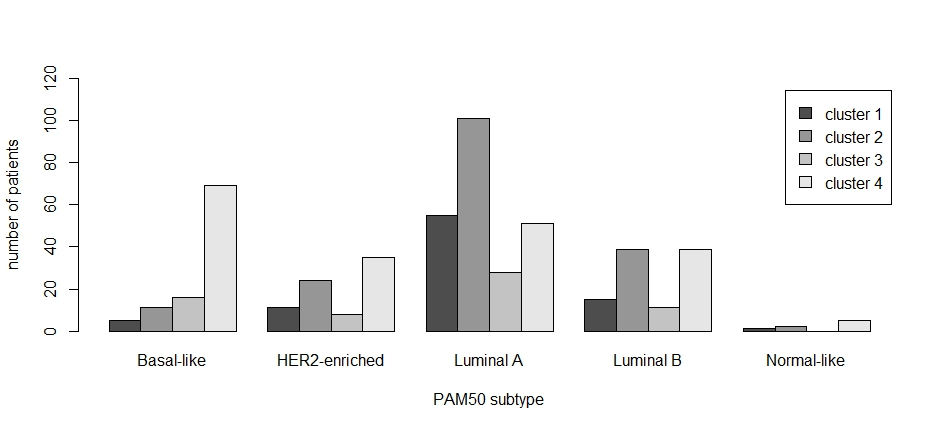
\includegraphics[scale=0.33]{images/Plot_clusters_per_subtype_4Groups.jpeg}
\captionsetup{font=small}
\captionof{figure}{Number of patients which are a member of each cluster, per PAM50 subtype.}
\label{fig:plot_clusters_subtype}
\end{figure}

\begin{figure}
\centering
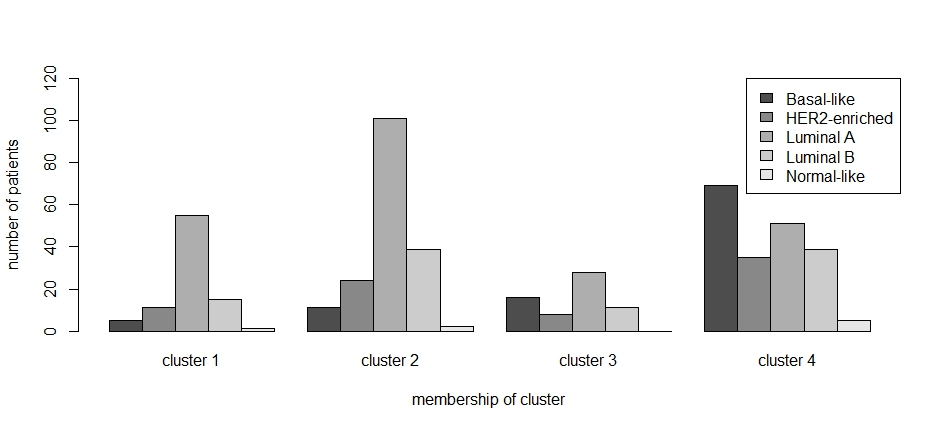
\includegraphics[scale=0.33]{images/Plot_subtypes_per_cluster_4Groups.jpeg}
\captionsetup{font=small}
\captionof{figure}{Number of patients with specific PAM50 subtype, per cluster.}
\label{fig:plot_subtypes_cluster}
\end{figure}

Research increasingly shows that a single type of cancer, for example breast cancer, is not one homogeneous disease. Instead, it can be divided in different \textit{subtypes} that display different harmful effects, and in turn require different treatment.
In order to validate the results of the clustering approach, we looked at the PAM50 tumor subtype classification \cite{parker2009supervised}, which was previously published for the patients in our records by the Cancer Genome Atlas Network \cite{cancer2012comprehensive}. PAM50 subtypes are determined by looking at the expression levels of 50 specific genes from a breast cancer sample in order to assign an \emph{intrinsic} subtype to the patient’s tumor. As this is based on expression data rather than the mutational gene data used in our clustering approach, correlation between the PAM50 subtypes and the identified clusters would be interesting as this would enable us to (partially) subtype breast cancer tumors based on gene mutation data. Furthermore, since the PAM50 tumor subtype classification has prognostic significance, correlation between the clusters and the PAM50 tumor subtypes would largely validate our clustering approach as being biologically relevant in a real-world cancer setting.
We analyzed the data by partitioning it into 4 non-overlapping clusters with a $\gamma$ of 0.5. We then assessed every patient in our dataset for membership of one or multiple clusters. A patient was considered a member of a specific cluster when that patient had at least one deleterious mutation (defined as a PHRED-scaled CADD score of at least 20 \cite{kircher2014general}). The results of this analysis are depicted in Figure \ref{fig:plot_clusters_subtype} and Figure \ref{fig:plot_subtypes_cluster}. We performed a $\chi$-square goodness of fit test on the distribution of the basal-like PAM50 subtype from Figure \ref{fig:plot_clusters_subtype} and on both the distributions of cluster 1 and cluster 2 from Figure \ref{fig:plot_subtypes_cluster} to test whether they deviated from a random assignment of patients to clusters. All three distributions deviated significantly from the random case (Basal-like: $\chi-squared = 103.48$, $df = 3$, $p-value < 2.2e-16$; cluster 1: $\chi-squared = 15.507$, $df = 4$, $p-value =0.003757$; Cluster 2: $\chi-squared = 22.388$, $df = 4$, $p-value = 0.0001678$).
Based on these results, and the observations from figure \ref{fig:plot_clusters_subtype} and figure \ref{fig:plot_subtypes_cluster}, two interesting conclusions could be drawn: 1) patients with a basal-like PAM50 tumor subtype were very likely to have a mutation in clustered pathway 4 and 2) patients with a mutation in pathway 1 or 2 were more likely to have a luminal A subtype. This shows that the identified gene clusters / pathways have at least some correlation with the PAM50 subtypes and could thus be useful in patient subtyping and exploring subsequent treatment options, although more research would be needed to confirm this. As such, our subtyping method is able to generate meaningful biological results in a cancer subtyping setting.



\section{conclusions and future work}
\label{sec:conclusion}
Motivated by a problem in bio-informatics, we presented a novel graph clustering problem involving two graphs, a co-occurrence graph whose weighted edges are part of the objective function, and an interaction graph with hard connectivity constraints. We propose two methods for handling the (potentially exponential in number) connectivity constraints, one based on enumerating all simple paths and the other being a cutting plane approach. We also present a number of extensions such as a bi-objective Pareto optimisation method to balance minimum cluster size and total penalty. Computational experiments show the properties of the different proposed methods, and a validation experiment on a separate biological data source demonstrates the potential of our proposed approach.

\bibliographystyle{IEEEtran}
\bibliography{references}

\end{document}

%%% Local Variables:
%%% mode: latex
%%% TeX-master: t
%%% End:
